\chapter{Standard Model and Supersymmetry}
\label{chap:SMSUSY}

This chapter presents an introduction to the Standard Model (SM) of particle physics, the theory that nowadays best described the subatomic world. In Section \ref{sec:smsusy:sm} a general overview of the SM is given. Section \ref{sec:smsusy:bsm} discusses the limitations of the SM, and some of the theoretical extensions proposed to overcome them. Finally Section \ref{sec:smsusy:susy} focuses on Supersymmetry (SUSY), one of the most promising of these extensions. Throughout this Chapter (as well as in the rest of this thesis) we use Natural units; we will thus use energy units to describe masses, as the speed of light ($c$) and the Plank constant ($\hslash$) are set to unity.


\section{The Standard Model of Particle Physics}
\label{sec:smsusy:sm}

The Standard Model (SM) is a renormalizable gauge quantum field theory based on the group $SU(3) \times SU(2) \times U(1)$. It has been developed in the second half of the 20th century \cite{Glashow:1961tr}\cite{Weinberg:1967tq}\cite{Salam:1980jd}, and since then the description that it gives of the elementary particles and of their interactions has been accurately tested by several experiments. Many experimental discoveries have been guided by the SM predictions, including the discovery of the top quark \cite{Abachi:1994td}\cite{PhysRevLett.74.2626} and up to the latest one, the observation of the Higgs boson at the LHC in July 2012 \cite{Aad:2012tfa}\cite{Chatrchyan:2012xdj}. 

\subsection{Particle Content of the Standard Model}

In the SM, particles are described as fields excitations. In the following sections, we introduce the quantum filed theory descriptions of fermions and bosons.

\subsubsection{Fermions}

Matter constituents are half-integer spin fields (\textit{fermions}). Fermions are further divided into two categories based on the type of interaction they experience:
\begin{itemize}
\item \textit{Leptons} experience only the electroweak interaction
\item \textit{Quarks} experience both the electroweak and the strong interaction
\end{itemize}

Both leptons and quarks come in three generations, and conventionally the numbering of these generations follows an order of increasing mass. While it is possible to observe free leptons, quarks exist only in bound states (\textit{hadrons}); this is because of confinement, discussed in Section \ref{sec:strong}. Hadrons built of three quarks have spin $\frac{1}{2}$ and are named \textit{barions}, while \textit{mesons} are formed by two quarks and have integer spin.


The free lagrangian of a fermion is given by:

\begin{equation}
 \mathcal{L}_{free} = \bar{\psi} \left( i \gamma^{\mu} \partial_{\mu} - m \right) \psi \, , \
 \label{eq:sm:dirac}
\end{equation}

\noindent where $\psi$ is the fermion field, $m$ its mass, $\gamma$ are the Dirac matrices and $\partial_{\mu}$ is the four-momentum derivative.


\subsubsection{Bosons}

Particles with integer spin are referred to as \textit{bosons}. In the SM, force carriers are described through spin-1 fields. 
The SM includes also a spin-0 particle, the Higgs boson. Is the interaction with the Higgs boson field that allows all the other elementary particles to acquire mass, as described in Section \ref{sec:smsusy:ew}.

The Klein-Gordon Lagrangian governs the kinenatic of spin-0 neutral particles:

\begin{equation}
\mathcal{L}_{free} = \frac{1}{2} \partial^\mu \phi \partial_\mu \phi + \frac{1}{2} m^2 \phi ^2 ,
\end{equation}

 
\noindent while in the case of charged particles (described through a complex filed) the Lagrangian becomes:

\begin{equation}
\mathcal{L}_{free} =  \partial^\mu \phi \partial_\mu \phi^* +  m^2 \phi \phi^* .
\end{equation}


\noindent The two equations above describe scalar particles. In the case of a vector filed, the expression of the Lagrangian is the following: 

\begin{equation}
\mathcal{L}_{free} =  - \frac{1}{4} F^{\mu \nu}F_{\mu \nu} +  \frac{1}{2} m^2 A^\mu A_\mu \, .
\label{eq:lproca}
\end{equation}

\noindent This is the Proca Lagrangian. In the case of a particle with zero mass, this reduces to the Maxwell Lagrangian:

\begin{equation}
\mathcal{L}_{free} =  - \frac{1}{4} F^{\mu \nu}F_{\mu \nu} ,
\label{eq:lmax}
\end{equation}


\noindent where $F^{\mu \nu} = \partial^\mu A_\nu - \partial^\nu A_\mu$.

\subsection{Interactions}

The SM describes all the interactions among elementary particles, except for gravity, for which nowadays no renormalizable quantum field theory is formulated. Table \ref{tab:sm_interazioni} presents a summary of the SM interactions and the properties of the corresponding force carriers. More details about the strong and electroweak sectors are given in the following sections.

\begin{table}[h]
\centering
\begin{tabular}{llccc}
\hline
\multirow{2}*{Interaction} & \multirow{2}*{Carrier} & \multirow{2}*{$\frac{Q}{e}$} & \multirow{2}*{Mass [GeV]} & \multirow{2}*{\textbf{$\alpha$}} \\
 & & & &  \\
\hline
\hline
Strong & Gluons (g)  & 0 & 0 & 10 \\
\hline
Electromagnetic & Photon ($\gamma$) & 0 & 0  & $10^{-2}$ \\
\hline
\multirow{2}*{Weak} & $W^{+}$, $W^{-}$    &  +1, -1 &  	$80.385$ $\pm0.015$ GeV   & \multirow{2}*{$10^{-6}$}\\
 & $Z^{0}$  & 0 &  	$91.1876$ $\pm0.0021$ GeV &  \\
\hline
\end{tabular}
\caption[Interaction in the Standard Model]{Interaction in the Standard Model. Here the different force carriers are listed, with their electric charges and masses \cite{pdg:rev}; $\alpha$ is the coupling constant of the different interactions.}
\label{tab:sm_interazioni}
\end{table}


\subsubsection{Gauge Invariance}

The interaction terms in the SM Lagrangian are introduced by promoting an already existing global symmetry of the Lagrangian ($\theta$) to a \textit{local} one ($\theta(x)$) function of the space-time coordinates. 
In general, given a Lagrangian globally invariant under a symmetry group, the fields transform as:
\begin{equation}
\psi \rightarrow e^{ig\theta_k \tau_k} \psi  
\end{equation}

\noindent where $\tau_k$ are the generators of the group and obey commutation relations: 
\begin{equation}
\left[ \tau_i, \tau_j \right] = i f_{ijk} \tau^k \, . \
\end{equation}

\noindent $f_{ijk}$ is the structure constant of the group and is always zero for Abelian groups. Promoting this invariance to a global one ($\theta_k \rightarrow \theta_k(x)$) implies adding to the theory:
\begin{itemize}
\item A number of massless gauge fields $W^\mu_k$ equal to the number of generators of the symmetry group, that transform as 
\begin{equation}
W^\mu_k \rightarrow W^\mu_k - \partial^\mu \theta_k - g \epsilon_{klm} \theta^m W^\mu_m 
\end{equation}
\item A covariant derivatibe: 
\begin{equation}
D^\mu = \partial^\mu + ig\tau^kW^\mu_k 
\end{equation}

\noindent that substitutes the standard derivative in the Lagrangian
\item A free Lagrangian for the vector fields as in Eq. \ref{eq:lproca}, with:
\begin{equation}
F^{\mu \nu}_k = \partial_\mu W_k^\nu - \partial_\nu W_k^\mu - g f_k^{lm} W^\mu_l W^\nu_m
\end{equation}
\noindent The last term, of second order in the field, is present only for non-Albelian symmetry groups. 
\end{itemize}


The SM is a theory invariant under $SU(3)_\mathrm{C} \times SU(2)_\mathrm{L} \times U(1)_\mathrm{Y}$. Imposing local invariance under $SU(3)_\mathrm{C}$ leads to the theory of strong interactions, while $SU(2)_\mathrm{L} \times U(1)_\mathrm{Y}$ is the symmetry whose breaking gives origin to the electroweak interactions. 

\subsubsection{Strong Interaction}
\label{sec:strong}

Quantum Chromo-Dynamics (QCD) is the theory that describes strong interactions, and it is invariant under the symmetry group $SU(3)_\mathrm{C}$, where the subscript C refers to the color, the quantum number associated with these interactions; this can assume three possible values denoted with red, blue and green. The observable states (hadrons) are color singlets, while quarks (anti-quarks) carry only one color (anti-colr) charge. Since the symmetry group is non-Abelian, also the corresponding eight gauge bosons (\textit{gluons}) carry a color charge (bi-color, with one color and one different anti-color) and therefore interact not only with quarks but also among themselves. Since $SU(3)_\mathrm{C}$ is believed to be an exact symmetry,  gluons are massless. 

The renormalization of a gauge theory leads to the definition of \textit{running coupling constants}, whose value depend on the energy scale where they are evaluated. In QCD, at leading order the dependence of the coupling constant from the energy scale is given by:

\begin{equation}
\alpha_\mathrm{s}(Q^2)=\frac{12\pi}{\left(11N_\mathrm{C}-2n_\mathrm{f}\right)\log{\frac{Q^2}{\Lambda_\mathrm{QCD}^2}}} 
\label{eq:alfaQCD}
\end{equation}

\noindent where $N_\mathrm{C}$ is the number of colors, $n_\mathrm{f}$ is the number of quark flavors that are active (i.e. whose mass is lower than the energy scale) and $\Lambda_\mathrm{QCD}$ is the infrared cutoff scale that sets the limit of validity of the perturbative approximation. In QCD $N_\mathrm{C} = 3$, so for $n_\mathrm{f}<16$ the coupling constants decreases with the increase of the energy scale of the process considered. This structure has important consequences on the properties of quarks and gluons:

\begin{itemize}
\item At high $Q^2$ ($\rightarrow$ small distances), $\alpha_\mathrm{s}$ becomes small enough for the perturbative approximation to be correct. In this case quarks and gluons behave as free particles (\textit{asymptotic freedom}) \cite{PhysRevLett.30.1343}\cite{PhysRevLett.30.1346}.
\item When the momentum transfer is small ($\rightarrow$ large distances) $\alpha_\mathrm{s}$ is large; this gives rise to \textit{confinement}: quarks can not be observed as isolated particles, as it is not possible to extract individual quarks from hadrons. When the distance between two quarks is increased, the potential energy increases as well, up to the point when is energetically more favorable to create from the vacuum a quark-antiquark pair and thus a new hadron is formed.
\item In a collider experiment, quarks and gluons will create a collimated spray of hadrons (\textit{jets})
\end{itemize}



\subsubsection{Electroweak Interaction and Higgs-Englert-Brout Mechanism}
\label{sec:smsusy:ew}

The theory of electroweak interactions is based on the symmetry group $SU(2)_\mathrm{L} \times U(1)_\mathrm{Y}$. This symmetry breaks at a scale around 100 GeV giving rise to the electromagnetic interaction, mediated by the photon, and to the weak interaction, mediated by the $Z$ (neutral currents) and $W^{\pm}$ bosons (charged currents). The number of mediators, four, is the same as the number of generators of the symmetry group. 

The $SU(2)_\mathrm{L}$ part of the symmetry group governs the weak interactions, and the suffix L indicates that only left-handed particles participate to them. Left-handed and right-handed fields ($\psi_L$ and $\psi_R$ respectively) are defined as:

\begin{equation}
\begin{aligned}
\psi_L = \frac{(1 - \gamma_5)}{2} \psi, \\
\psi_R = \frac{(1 + \gamma_5)}{2} \psi
\end{aligned}
\label{eq:sm:LR}
\end{equation}

\noindent where $(1 \pm \gamma_5)/2$ are the chirality projectors, and $\gamma_5$ is defined as $\gamma_5 = i \gamma^0 \gamma^1 \gamma^2 \gamma^3 $. Looking back at Eq. \ref{eq:sm:dirac}, it can be noted that, if we decompose the fermion filed into its left-handed and right-handed components, the derivative term keeps $\psi_L$ and $\psi_R$ separated, while the mass term mixes them:
\begin{equation}
-m \bar \psi \psi = -m \bar \psi P_L^2 \psi - m \bar \psi P_R^2 \psi
	= -m \bar \psi_R \psi_L - m \bar \psi_L \psi_R \
\end{equation}


The covariant derivative for the  $SU(2)_\mathrm{L} \times U(1)_\mathrm{Y}$ group is:
\begin{equation}
\mathcal{D}^{\mu} = \partial^{\mu} + i \frac{g'}{2} B^\mu Y + ig W^\mu_k T^k
\label{eq:sm:covD}
\end{equation}

\noindent and substituting with this the regular derivative results in the interaction Lagrangian:
\begin{equation}
\mathcal{L}_{int}^{EW} = -\frac{g'}{2} \left( \bar{\psi} \gamma_\mu Y \psi \right) B^\mu - g \sum_k \left( \bar{\psi} \gamma_\mu T^k \psi  \right) W_k^\mu
\end{equation}

\noindent where we have introduced $T^k$, the weak isospin operator, and $Y$, the hypercharge operator, and the respective coupling constants $g$ and $g'$. The quantum numbers of the $T^k$ and $Y$ operators relate to the electric change $Q$ through the  Gell-Mann Nishijima relation:

\begin{equation}
Q = \frac{Y}{2} + T_3
\label{eq:sm:Q}
\end{equation}

\noindent where $Y$ is the hypercharge quantum number and $T_3$ is the quantum number of the third component of the isospin. 

In the case of an $SU(2)$ symmetry, is not possible to add directly to the lagrangian a mass term for the vector bosons of the form in Eq. \ref{eq:lproca}, as it would spoil the $SU(2)$ local invariance. The Higgs-Englert-Brout mechanism \cite{Englert:1964et}\cite{Higgs:1964pj}\cite{Higgs:1964ia} solves this problem through Spontaneous Symmetry Breaking (SSB) of the $SU(2)_\mathrm{L} \times U(1)_\mathrm{Y}$ invariance. The SSB is obtained by adding to the theory one extra isospin doublet of complex scalar components (\textit{Higgs field}):

\begin{equation}
	\Phi = \left( \begin{array}{c} \phi^+  \\ \phi^0 \end{array} \right)
\end{equation}
%	= \frac{1}{\sqrt{2}} \left( \begin{array}{c} \phi_1 + i \phi_2 \\ \phi_3 + i \phi_4 \end{array} \right)

This doublet has hypercharge Y=1 and isospin $T=\frac{1}{2}$; the first component is positively charged, while the second one is electrically neutral. The Lagrangian for this new field includes a kinetic and a potential term:

\begin{equation}
	\mathcal{L}_{\Phi} = ( \mathcal{D}_{\mu} \Phi)^{\dagger} (\mathcal{D}^{\mu} \Phi) - V(\Phi) 
	\label{eq:Lhiggs}
\end{equation}

\noindent where $\mathcal{D}_{\mu}$ is the covariant derivative defined in Eq. \ref{eq:sm:covD} and the potential $V(\Phi)$ is given by:

\begin{equation}
 V(\Phi) = - \mu^2 \Phi^{\dagger} \Phi + \lambda (\Phi^{\dagger} \Phi)^2 \, . \
	\label{eq:hpot}
\end{equation}

\noindent The two real parameters $\mu^2$ and $\lambda$ relate respectively to the mass term and the strength of the self-interaction term. The shape of the potential depends on the value of these parameters:
\begin{itemize}
\item If $\lambda < 0$, the potential does not present any stable minima, and is therefore unphysical.
\item If $\lambda > 0$ and $\mu^2 > 0$ there is only one solution to the minimization of the potential, $\Phi=0$. This case is shown in Fig. \ref{fig:sm:higgsV}(a).
\item If $\lambda > 0$ and $\mu^2 < 0$, the field acquires a vacuum expectation values (VEV) as the minima is not at zero; it lies instead on the points of the circumference such that:
\begin{equation}
\Phi^{\dagger} \Phi = \frac{\mu^2}{2 \lambda}  \equiv \frac{v^2}{2}
\end{equation}
\noindent Fig. \ref{fig:sm:higgsV}(b) illustrates this case.
\end{itemize}


\begin{figure}[ht]
\centering
\subfigure[]{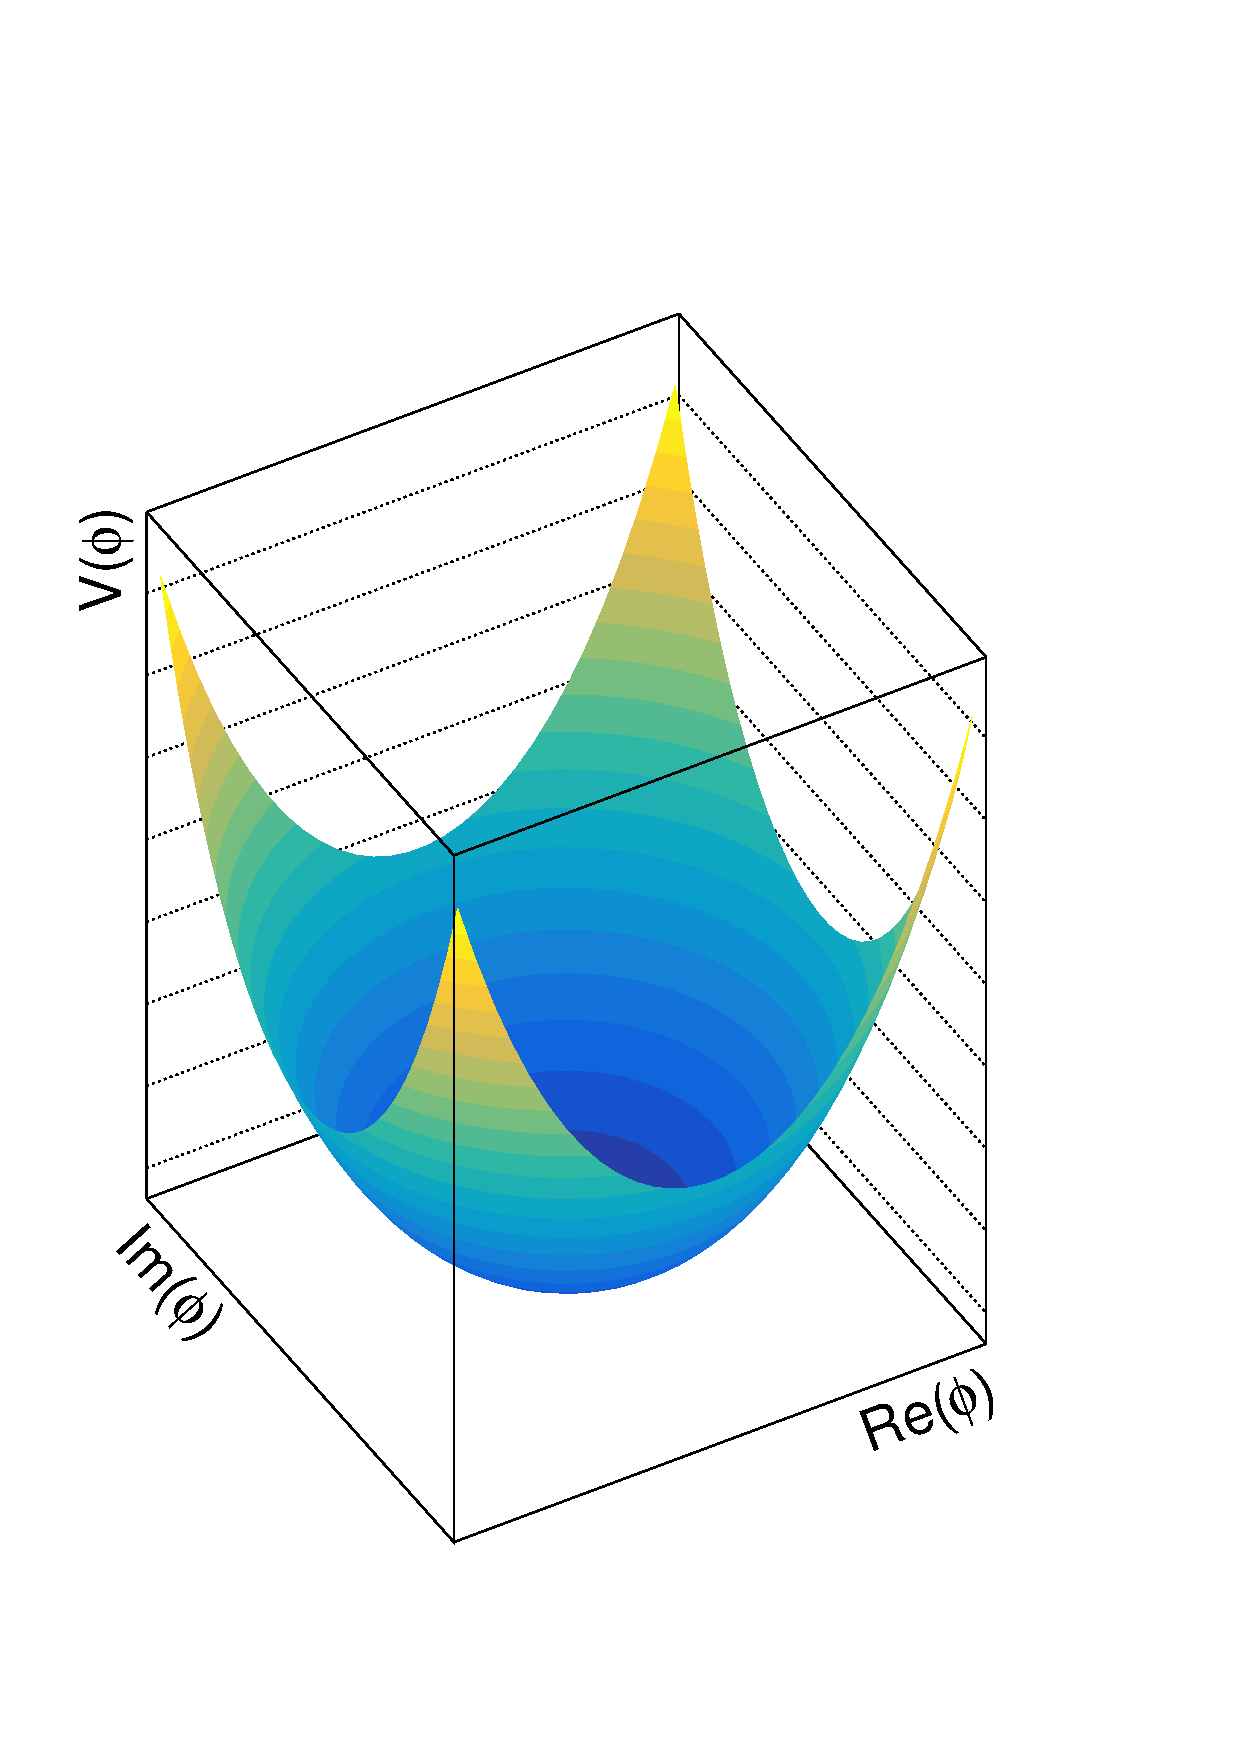
\includegraphics[width=0.49\textwidth]{produce_plots/sm/higgs_posmu2.pdf}}
\subfigure[]{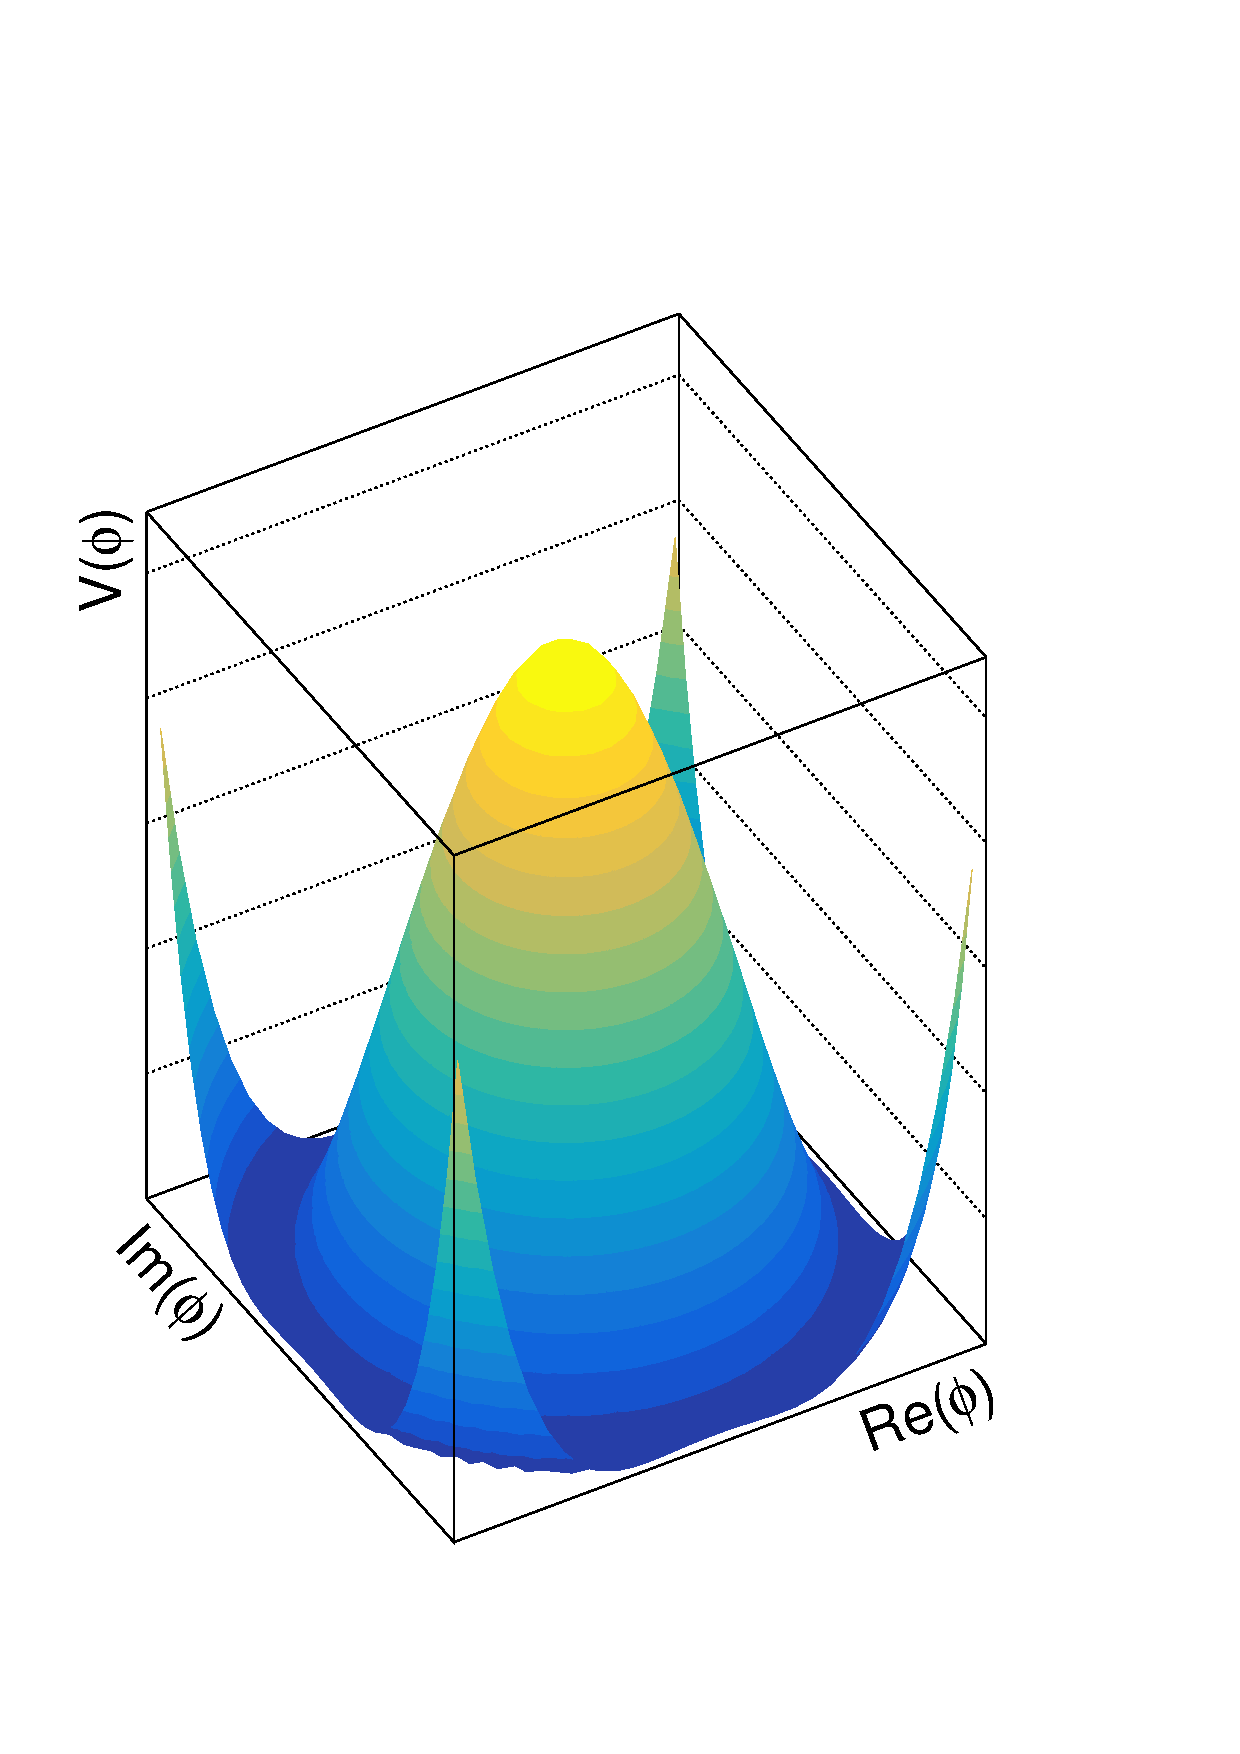
\includegraphics[width=0.49\textwidth]{produce_plots/sm/higgs_negmu2.pdf}}
\caption{Higgs potential in the case $\lambda > 0$ and $\mu^2 > 0$ (a) and $\lambda > 0$ and $\mu^2 < 0$ (b).}
\label{fig:sm:higgsV}
\end{figure}

Up to this point the $SU(2)_\mathrm{L} \times U(1)_\mathrm{Y}$ symmetry is still intact, but the explicit choice of one of the infinite possible vacuum states for the Higgs field breaks the symmetry. According to the Goldstone theorem \cite{Goldstone:1962es}, the breaking of a continuous symmetry leads to the appearance of new massless scalar particles as allowed excitations. These new degrees of freedom can be absorbed by the existing gauge bosons, thus giving them mass. To meet the experimental requirement of a massless photon, the choice of the Higgs vacuum has not to break the electromagnetic symmetry ($U(1)_{EM}$), so the component of the Higgs doublet that acquires a VEV is the neutral one:

\begin{equation}
	\Phi_0 = \frac{1}{\sqrt{2}} \left( \begin{array}{c} 0 \\ v  \end{array} \right) \, . \
\label{eq:hvphi}
\end{equation}

We can then expand small excitations around the minimum:

\begin{equation}
	\Phi = \frac{e^{i \vec{\sigma} \cdot \vec{\theta}(x)/v }}{\sqrt{2}} \left( \begin{array}{c} 0 \\ v + \phi(x) \end{array} \right) \, . \
\label{eq:hvphi}
\end{equation}

\noindent where $\phi(x)$ is the physical field associated with the Higgs boson, and $\vec{\theta}(x)$ the three degrees of freedom absorbed to give masses to the $Z$ and $W^\pm$ bosons. Inserting Eq. \ref{eq:hvphi} in Eq. \ref{eq:Lhiggs} relates the mass of the Higgs boson to the parameters in the potential:
\begin{equation}
m_H = \sqrt{- 2 \mu^2} = \sqrt{2 \lambda} v
\label{eq:sm:higgsmass}
\end{equation}

Since the numeric value of the $\mu^2$ and $\lambda$ parameters is not set, the theory does not predict a specific value for $m_H$. The $(\mathcal{D}_{\mu} \Phi)^{\dagger} (\mathcal{D}^{\mu} \Phi)$ term in Eq. \ref{eq:Lhiggs} gives rise to the physical mass of the gauge boson, that at tree level are:

\begin{equation}
\begin{aligned}
m_\gamma &= 0 \, ,\\
m_Z &= \frac{v \sqrt{g^2 + g'^2}}{2} \, , \\
m_W &= \frac{vg}{2} =  \cos\theta_W m_Z \, ,
\end{aligned}
\end{equation}

\noindent where we have introduced the Weinberg angle $\theta_W$ such that:
\begin{equation}
\tan\theta_W \equiv \frac{g'}{g}
\end{equation}

The physical mass eigenstates of the gauge bosons are a rotation of the interactions eigenstates, given by:

\begin{equation}
\begin{aligned}
W_\mu^\pm &= \frac{W_\mu^1 \mp W_\mu^2}{\sqrt{2}} \, , \\
A_\mu &= B_\mu \cos\theta_W + W^3_\mu \sin\theta_W \, ,  \\
Z_\mu &= W^3_\mu \cos\theta_W - B_\mu \sin\theta_W \, .
\end{aligned}
\label{eq:wein}
\end{equation}

The Higgs-Englert-Brout mechanism generates automatically a mass term for the gauge bosons, that does not break the global underlying $SU(2)_\mathrm{L} \times U(1)_\mathrm{Y}$ symmetry. The Higgs field is used also to make fermion mass terms arise, but in this case it is necessary to add the couplings by hand. The fermion masses are assumed to be proportional to the strength of the coupling and, unlike what happens with the masses of the gauge bosons, they are not related to other parameters of the theory. While the Higgs filed itself is enough to give mass to down-type fermions, the mass term for the down type ones requires the introduction of the complex conjugate of the Higgs field ($\Phi_C$):

\begin{equation}
 \Phi_C = i \sigma^2 \Phi^* 
	= i \left( \begin{array}{cc} 0 & -i \\ i & 0 \end{array} \right) 
	\left( \begin{array}{c} \phi^- \\ \phi^{0*} \end{array} \right)
	= \left( \begin{array}{c} \phi^{0*} \\ - \phi^- \end{array} \right)
\end{equation}

If we identify as $g_f$ the coupling of the fermion $f$ to the Higgs field (\textit{Yukawa coupling}), the additional part of the Lagrangian that generates the fermion masses is:

\begin{equation}
\begin{aligned}
\mathcal{L}_{Yukawa} &= - \left[  y_d \left( \bar{u}_L \,\, \bar{d}_L  \right) \Phi d_R +  y_u \left( \bar{u}_L \,\, \bar{d}_L  \right) \Phi_C u_R \right] + h.c. \\
&= - \frac{1}{\sqrt{2}} \left[  y_d \left( v + \phi \right) \bar{d}_L d_R + h.c. + y_u \left( v + \phi \right) \bar{u}_L d_u + h.c. \right] 
\end{aligned}
\end{equation}

\noindent In this equation we can now easily identify the fermion mass terms, of the form:

\begin{equation}
m_f =  \frac{1}{\sqrt{2}} v y_f
\end{equation}

The matrices $y_f$ are not necessarily diagonal, but they can be diagonalized through a unitary transformation, that we can interpret as the transformation that relates the mass eigenstates to the weak interaction eigenstates. In the quark sector, this transformation is encoded in the Cabibbo–Kobayashi–Maskawa (CKM) matrix \cite{Cabibbo:1963yz}\cite{Kobayashi:1973fv}, that describes the mixing of the down-type quarks. In the SM with three generations of fermions, the CKM matrix is specified by three angles and one complex phase, that can induce CP-violation.


\section{Limits of the Standard Models and its Extensions}
\label{sec:smsusy:bsm}

Despite its undeniable success in describing the subatomic world, the SM has some limitations that lead scientists to consider it the low-energy limit of a more general theory. Nowadays there is no perfect candidate to fill the role of this general theory, but the shortcomings of the SM highlight the characteristics this theory should have. Section \ref{sec:sm:missingpieces} discusses the experimental observations that are not enclosed in the SM framework, whose lacking is an objective limit of the SM. In section \ref{sec:sm:aesthetics} we review some other features that the SM is missing that, while not being strictly necessary, would be desirable in a general theory. Some theories and models candidate to extend the SM are briefly presented in Section \ref{sec:sm:extensions}.

\subsection{Missing Pieces}
\label{sec:sm:missingpieces}

The SM lacks an explanation for some well established experimental phenomena. 

\subsubsection*{Neutrino Masses}

Neutrino oscillations \cite{PhysRevLett.81.1562} are possible only if there is a mass difference between the three neutrino generations, which automatically implies non-zero masses for at least some neutrinos. Although neutrino mass terms could be added to the SM through right-handed neutrinos or a description of neutrinos as Majorana particles, the plain SM describes neutrinos as massless particles.

\subsubsection*{Dark Matter and Dark Energy}

The SM describes only baryonic matter; this accounts for only 5\% of the universe composition. Even though no direct observation of it has been made so far, we know there is also another type of matter, that does not participate to electroweak interactions and  accounts for about 27\% of the universe composition.  Since this type of matter does not reflect light, it is known as \textit{dark matter}. The presence of dark matter has been postulated for the first time from the rotational velocity of galaxies \cite{Zwicky:1937zza}, but this evidence has now been confirmed also by other observations, including the analysis of the cosmic microwave background from the WMAP and Plank collaborations \cite{Larson:2010gs} \cite{Ade:2013zuv}. The sum of baryonic and dark matter describes about 32\% of the universe. The remaining part is the energy responsible for the accelerated expansion of the universe, \textit{dark energy}. While some extensions of the SM provide candidates for dark matter, at the moment no theory provides one for dark energy.


\subsubsection*{CP Violation}

CP-violating processes are needed in order to produce asymmetry between the matter and the anti-matter content of our universe. While the SM provides one source of CP violation with the complex phase in the CKM matrix mentioned in Section \ref{sec:smsusy:ew}, this is not enough and additional sources are needed in order to explain the observed asymmetry.

\subsubsection*{Gravity}

Gravity is the only force acting on elementary particles that is not described by the SM. In fact, not only is not described by the SM, but the simple attempt to quantize gravity through a spin-2  mediator (\textit{graviton}) leads to a non-renormalizable theory. The strength of gravity is expected to be comparable to the one of the other forces at the \textit{Plank scale} ($\Lambda_{Plank}$, $10^{19}$ GeV). 

\subsection{Aesthetic Shortcomings}
\label{sec:sm:aesthetics}

While the previous section discusses objective limits of the SM, there are also some aesthetic criteria that the SM does not seem to satisfy. These are mostly based on the concept of \textit{Naturalness}: unless there is a good reason, the parameters of a "beautiful" theory should be all of the same order of magnitude, and a theory where instead the parameters are bound to assume very specific and different values (\textit{fine tuning}) seems "unnatural". It is important to notice that this naturalness requirement is subjective, as well as the amount of fine tuning that we judge to be too much for a theory to be considered natural.


\subsubsection*{Hierarchy Problem and Higgs Mass}

The expression for the mass of the Higgs boson in Eq. \ref{eq:sm:higgsmass} contains only the tree level component. The proper computation should include the radiative contributions from all the particles that couple with the Higgs boson, directly or indirectly. A fermion, whose Yukawa coupling is given by $-\lambda_f \phi \bar{f} f$, will lead to a correction to the Higgs mass with a divergent integral; this can be computed for example with a cut-off regularization, and in this case the resulting correction to the Higgs mass, shown in Fig. \ref{fig:sm:h_corr}(a), is:
\begin{equation}
\Delta m_H^2 \>=\>  
-{|y_f|^2\over 8 \pi^2} \Lambda_{UV}^2 + \mathcal{O}(\ln \Lambda_{UV} )
\label{eq:divhf}
\end{equation}

where $\Lambda_{UV}^2$ is the cut-off scale, identified with the limit of validity of the theory. If we assume that no physics beyond the SM (BSM) is present up to $\Lambda_{Plank}$, having corrections to the mass proportional to $\Lambda_{UV}$ requires a fine tuning of the parameters of the order of $\frac{m_H}{\Lambda_{UV}} \approx 10^{-17}$. This is due to the strong hierarchy of the scales involved (\textit{hierarchy problem}) \cite{Weinberg:1975gm}\cite{PhysRevD.20.2619}\cite{PhysRevD.14.1667}\cite{tHooft:1979rat}. Since the correction to the mass is proportional to the Yukawa coupling of the fermion, it is clear that the most important correction is the one given by the top quark, whose Yukawa coupling is $y_t \approx 0.996$. 

Despite this, it can still be argued that the appearance of the $\Lambda_{UV}$ divergence is connected more to the regularization schema rather than the theory itself. But even in this case, the value of 125 GeV for the Higgs mass remains difficult to justify. The The SM Lagrangian does not have any symmetry that prevents the Higgs boson to couple to new BSM particles. If we assume the existence of a complex scalar that couples with the Higgs field through $ -y_S|\phi|^2 |S|^2$, the correction to the Higgs propagator, shown in Fig. \ref{fig:sm:h_corr}(b), is given by:

\begin{equation}
\Delta m_H^2 \>=\> {y_S\over 16 \pi^2}
\left [\Lambda_{UV}^2 - 2 m_S^2
\> {\rm ln}(\Lambda_{UV}/m_S) + \ldots
\right ].
\label{eq:divhs}
\end{equation}

Beside the first term, proportional to $\Lambda_{UV}^2$, that can be thought as a consequence of the cut-off regularization, we also have a second  term proportional to $m_S^2$. If we assume that BSM physics exists and that, since it has not yet been observed, $m_S$ must be large, this contribution drives $m_H$ to high values. A similar argument applies even if the new BSM sector and the Higgs filed do not couple directly but, for example, share a gauge interaction.

\begin{figure}[ht]
\centering
\subfigure[]{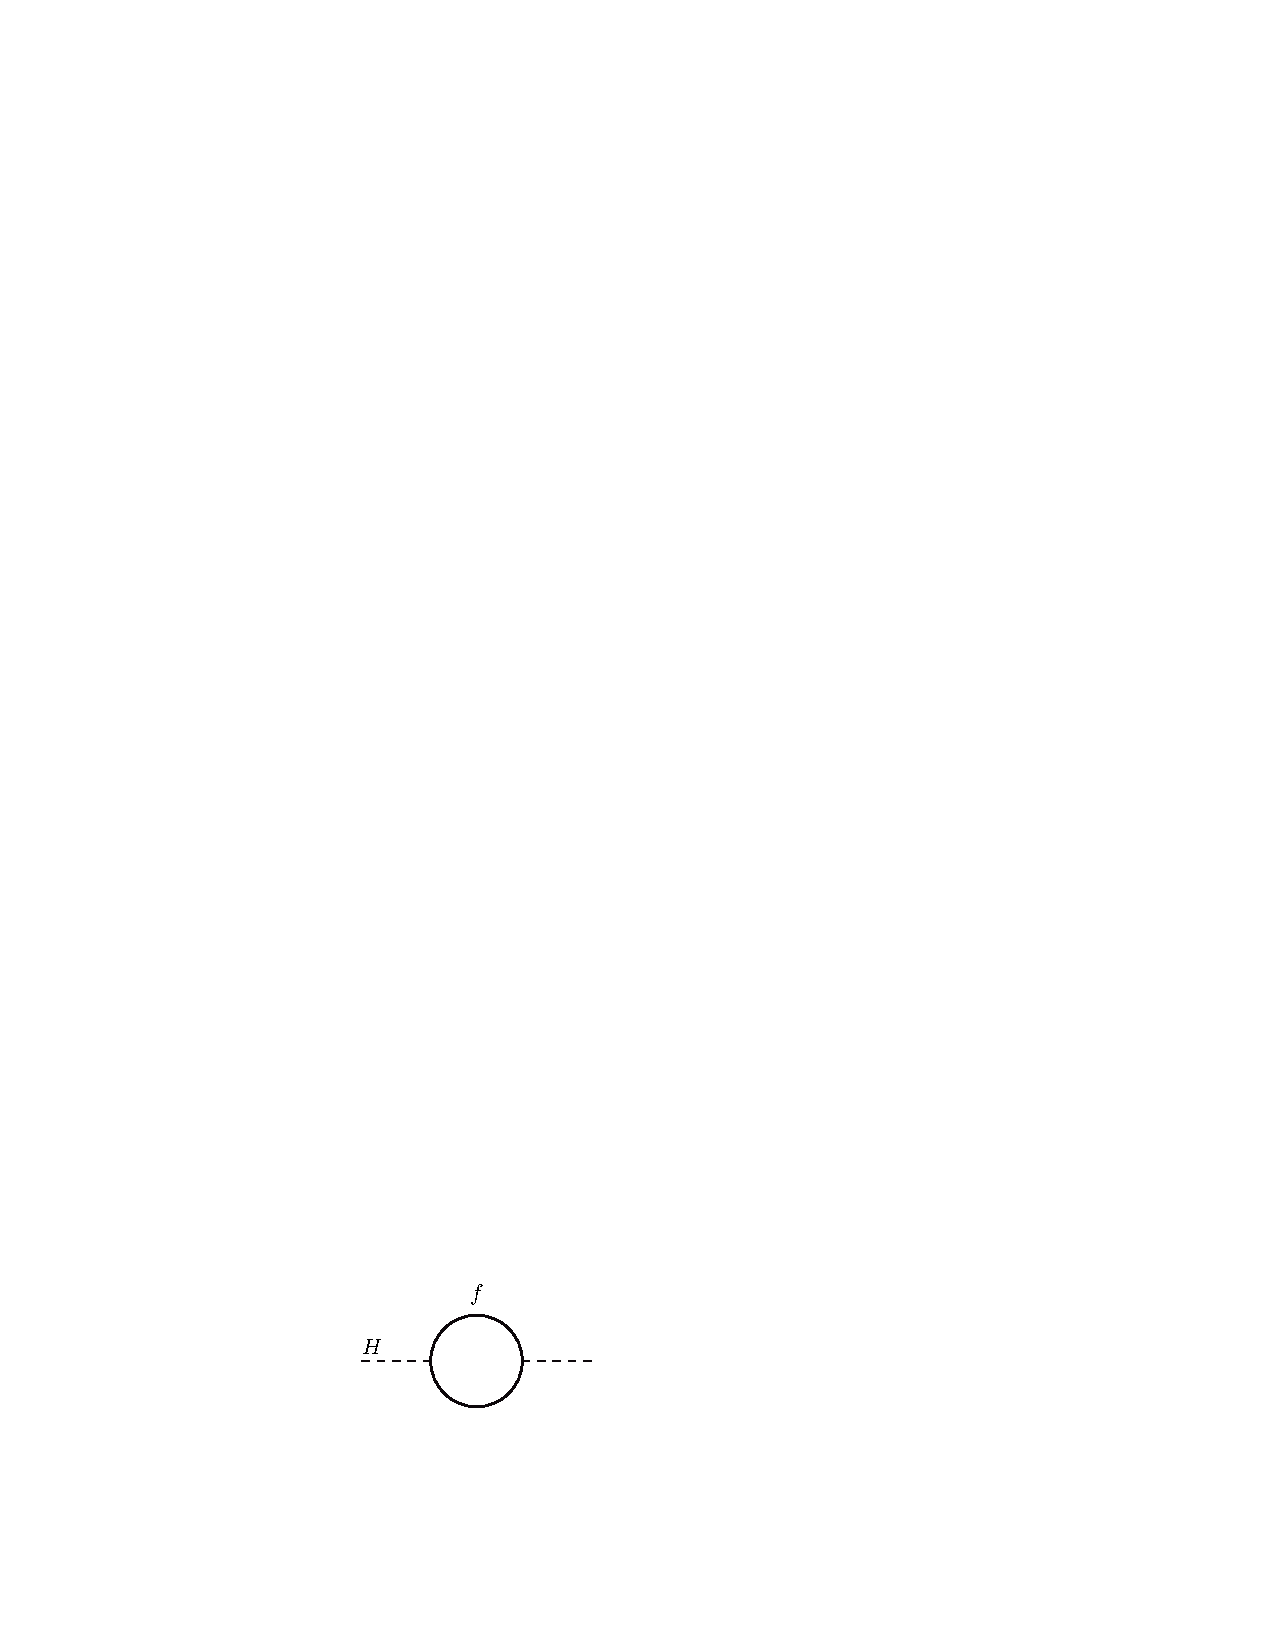
\includegraphics[width=0.36\textwidth]{figures/theory/h_corr_f.pdf}}
\subfigure[]{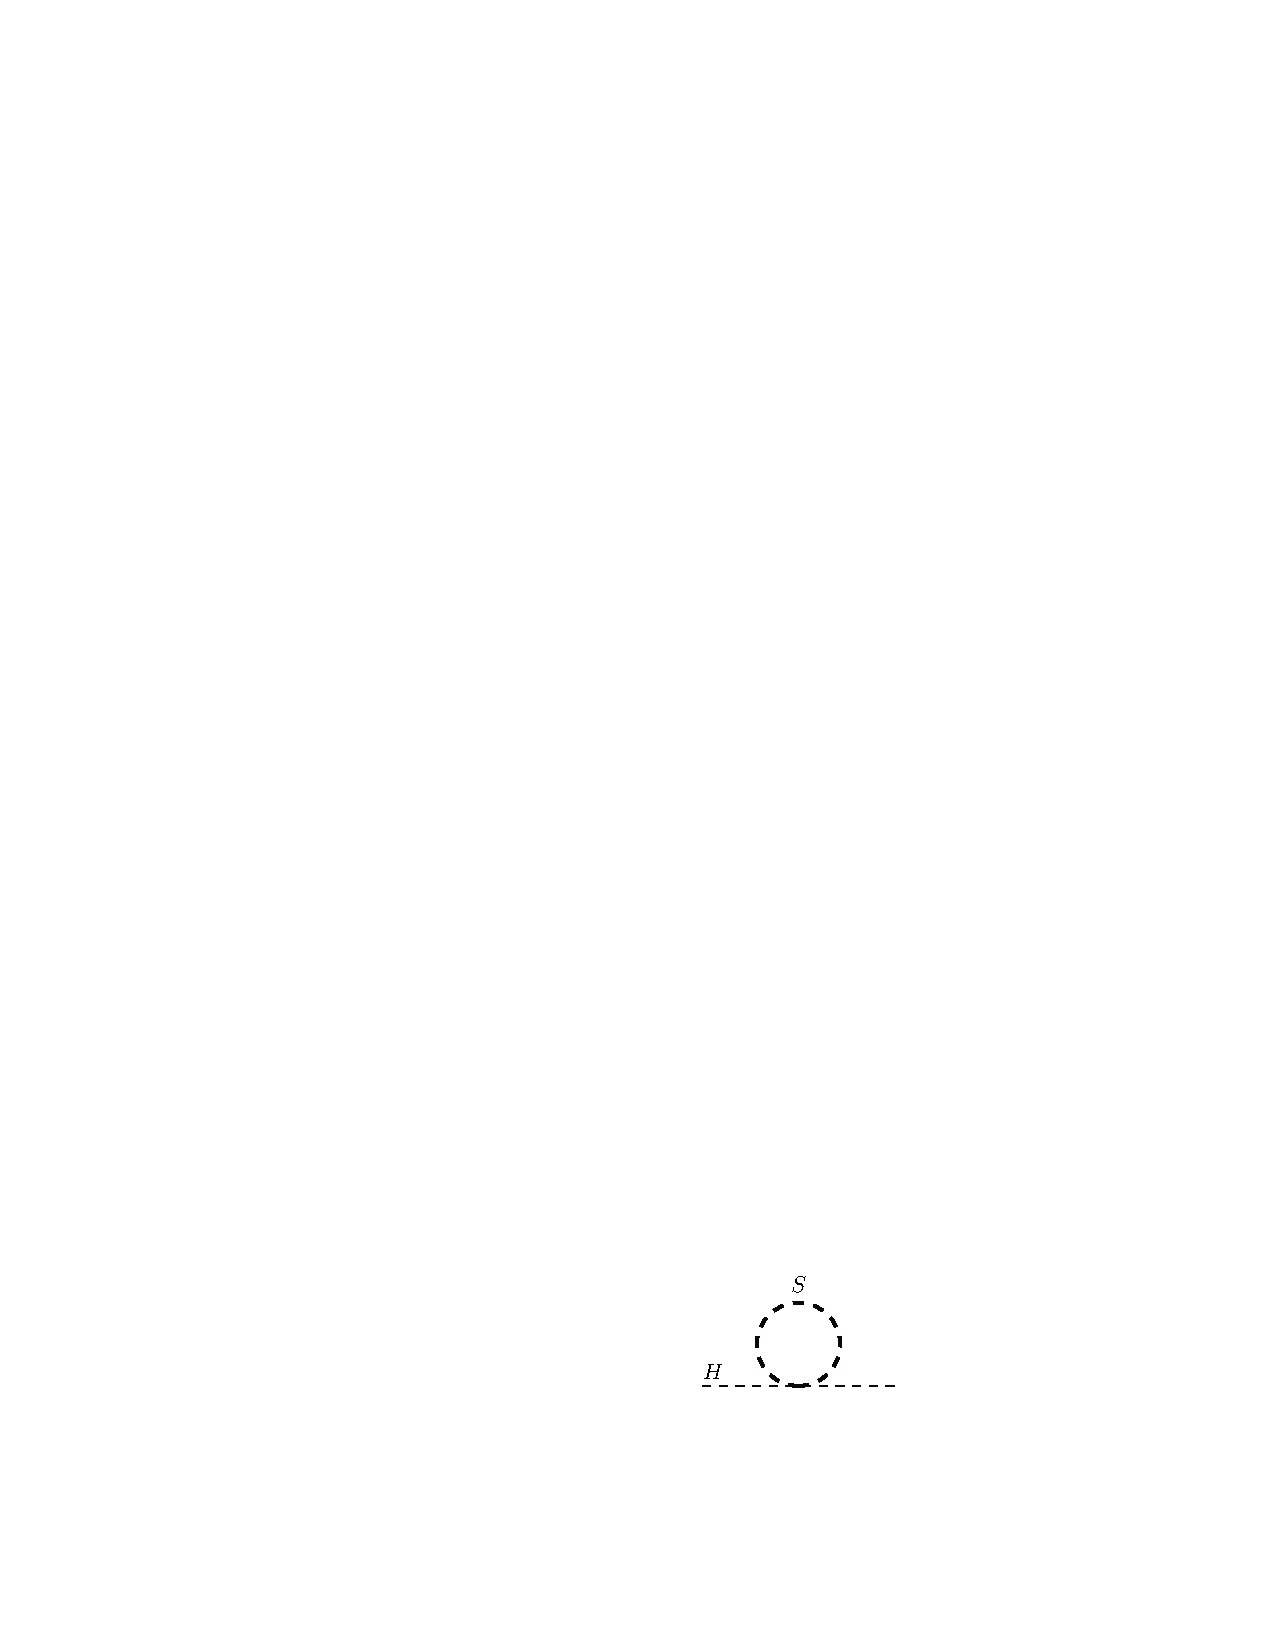
\includegraphics[width=0.36\textwidth]{figures/theory/h_corr_s.pdf}}
\caption{Correction to the Higgs boson propagator form the interaction with a fermion (a) and with a scalar (b), figure from Ref. \cite{Martin:1997ns}.}
\label{fig:sm:h_corr}
\end{figure}

\subsubsection*{Fermion Hierarchy Problem} 

Fermion masses are less sensitive than the Higgs mass to the cut-off scale as the divergence is only logarithmic. Nevertheless, it is striking how strong the fermion Yukawa coupling hierarchy is: even if we don't consider neutrinos, fermion masses span about six order of magnitudes, without any apparent reason

\subsubsection*{Unification of Coupling Constants}

The SM coupling constants of the $SU(3)_\mathrm{C}$, $SU(2)_\mathrm{L}$ and $U(1)_\mathrm{Y}$ groups have a different evolution, and the extrapolation of their values at very high energies suggests a common value at a scale $M_{GUT} \approx 10^{15}-10^{16}$ GeV, after which the different couplings unite. If the only particles involved in the computation of the evolution of the coupling constants are the SM ones, there is no exact crossing point, as shown in Fig. \ref{fig:susy:gut}(a).

\subsection*{Strong CP Problem}

The most general SM QCD Lagrangian should include also a CP-violating angle, and this would not spoil renormalizability. The presence of this term would have directly measurable physical consequences, for example a non-zero electric dipole moment for the neutron (nEDM). The tight  limits on the nEDM ( $< 3.6 \times 10^{-26}$ e cm at 95\% CL \cite{PhysRevD.92.092003}) translate into upper limits on the parameter regulating the CP-violating term of the QCD Lagrangian ($< 10^{-10}$ rad), while there is no theoretical reason why it should not be of order 1. 


\subsection{Standard Model Extensions}
\label{sec:sm:extensions}

The aspects of the particle physics world not yet described by the SM, are an indication that the SM should be extended.
In this section we briefly discuss some of the most popular theories and models proposed to extend the SM, except from Supersymmetry which is discussed in more details in section \ref{sec:smsusy:susy}. These extensions introduce typically one or more of the following:

\begin{itemize}
\item New particles, that can be independent particles or "partners" of the SM ones.
\item New symmetries, that can be broken 
\item New degrees of freedom, such as new quantum numbers or extra dimensions.
\item New forces, whose strength depends on the energy scale
\end{itemize}

\subsubsection*{Little Higgs}
% chiara: expand
Little Higgs models address the problem of the Higgs mass by considering the Higgs boson as a pseudo-Goldstone boson of a global symmetry. This leads to a light mass for the Higgs like it does for the pion in QCD.

\subsubsection*{Technicolor}
In technicolor models \cite{Weinberg:1975gm}\cite{PhysRevD.20.2619} the mass of the $Z$ and $W^{\pm}$ bosons is not generated through the interaction with the Higgs boson, but dynamically with a new asymptotically free gauge interaction whose strength is higher at small distances; the analogy with QCD (and the "color" degree of freedom) lead to the name technicolor. New fermions ("technifermions") are also introduced, transforming under the group vectorial representation. The Higgs boson is not predicted by technicolor, but it can be included in the models as a singlet scalar resonance, a dilaton, or a singlet pseudo-Goldstone boson.

\subsubsection*{Extra Dimensions}

The first attempt to introduce additional spacial dimensions to unify forces was done in the 1920's by Kaluza and Klein \cite{Kaluza}\cite{Klein:1926tv}, who interpreted our four-dimensional universe as a "brane" of a higher-dimensional spacetime. While the SM foresees only three spatial dimensions, adding extra dimensions can explain the observed weakness of gravity with respect to the other forces as it would be diluted in the extra dimensions. 
% rephrase
Particles propagating in the extra dimensions manifest in our brane as Kaluza-Klein modes. % end rephrase
While the first model from Kaluza and Klein was disproved shortly afterwards, similar ideas and formalism have been used also afterwards:  

\begin{itemize}
\item In the Arkani-Hamed-Dimopoulos-Dvali (ADD) model \cite{ArkaniHamed:1998rs}, two (or more) extra dimensions are added in which only gravity can propagate (through a graviton).
\item In the Randall and Sundrum model \cite{PhysRevLett.83.3370} the universe is conceived as five-dimensional Anti-de Sitter spacetime, and the weakness of gravity is explained through red-shift of the gravity brane.
\end{itemize}


\section{Supersymmetry}
\label{sec:smsusy:susy}

Supersymmetry (SUSY) \cite{Wess:1974tw}\cite{Salam:1974ig} is an extension of the Poincar\'e group that rotates bosonic states into fermionic ones and vice versa, through the supercharge operator ($Q$) that carries itself a fermionic charge: 

\begin{equation}
Q |{\rm boson}\rangle = |{\rm fermion }\rangle \qquad\qquad
Q |{\rm fermion}\rangle = |{\rm boson }\rangle 
\end{equation}

The Haag-Lopuszanski-Sohnius extension of the Coleman-Mandula theorem \cite{HAAG1975257} allows such operator as only non-trivial extension of the Poincar\'e in a consistent four-dimensional theory, as the operator and his hermitian conjugate ($Q^\dagger$) satisfy the following relations:

\begin{equation}
\begin{aligned}
&\{ Q, Q^\dagger \} = P^\mu ,  \\
&\{ Q,Q \} = \{ Q^\dagger , Q^\dagger \} = 0 ,  \\
&[ P^\mu , Q  ] = [P^\mu, Q^\dagger ] = 0 ,
\label{eq:susyalgth}
\end{aligned}
\end{equation}

where $P$ is the four-momentum operator. These relations, that define the Superssymmetry algebra, make it clear how the action of the supercharge is related to the Poincar\'e group: the combination of two supersymmetry rotations is a space-time translation.

\subsubsection{Supermultiplets}

The irreducible representations of the SUSY algebra are the \textit{supermultiplets}, that contain both bosons and fermions. Particles within the same supermultiplet are known as \textit{superpartners} of each others. Superpartners of the SM particles are indicated with the same letter but with a $\sim$ on top of it. Depending on their particle content, supermultiplets are classified into:

\begin{itemize}
\item \textit{Chiral supermultiplets} are the ones containing the SM fermions and their superpartners. Each Dirac fermionic filed can be seen as two separate Weyl filed, each of which has two degrees of freedom and is associated with a complex scalar as a superpartner. The name given to superpartners of fermions is \textit{sfermions} (e.g. the superpartner of the top is the stop). Since chiral supermultiplets are formed by spin-0 and spin-$\frac{1}{2}$ particles, they contain also the SUSY extended Higgs sector, as described in Section \ref{sec:susy:higgs}.

\item \textit{Gauge supermultiplets} contain gauge bosons and their superpartners. Each spin-1 SM boson is associated to a spin-$\frac{1}{2}$ Weyl fermion, as before the electroweak symmetry breaking all the gauge bosons are massless and have only two degrees of freedom. The name of the superpartners of the gauge bosons is the same as the corresponding SM particle but with a -ino suffix (e.g. the gluon superpartner is the gluino). 

\item \textit{Gravitational supermultiplets}. If we assume that gravity is mediated by the graviton, then a third type of supermultiplet is necessary that contains spin-2 graviton and its superpartner, the spin-$\frac{3}{2}$ gravitino.

\end{itemize}

% Avoid fine tuning

% SUSY is a broken symmetry
\subsubsection{SUSY and the Higgs Mass}

Superpartners share the same electric charge, isospin and QCD color as $Q$ and $Q^\dagger$ commute with the generator of the gauge transformations.
The third equality in \ref{eq:susyalgth} implies that $[ (P^\mu)^2 , Q  ]=0$. If we think of this as an operator applied to a supermultiplet, this implies that all the particles within the same supermultiplet should have also the same mass. The superpartners also bring a radiative correction to the Higgs mass, since they couple to the Higgs with the same coupling constant as their SM partners ($y_S=y_f=y$). If we consider the case of a fermion and a sfermion, according to Eq. \ref{eq:divhf} and Eq. \ref{eq:divhs} the two contributions have opposite sign and the total correction is:

\begin{equation}
\Delta m_H^2 \>=\> {y\over 16 \pi^2}
\left [ m_f^2
\> {\rm ln}(\Lambda_{UV}/m_f) 
- m_S^2
\> {\rm ln}(\Lambda_{UV}/m_S) 
\right ].
\label{eq:divhsusy}
\end{equation}

This correction cancels if each SM particle and its superpartner have the same mass. Unfortunately we know that, if SUSY exists, it must be a broken symmetry as the superpartners do not have the same mass as the corresponding SM particles (otherwise they would have been already observed). Since the correction to the Higgs mass becomes larger with the increase of the mass difference between particles in the same supermultiplet, SUSY remains a solution to the Higgs hierarchy problem as long as this mass difference is reasonably small.


% Unifications of the coupling constants

\begin{figure}[ht]
\centering
\subfigure[]{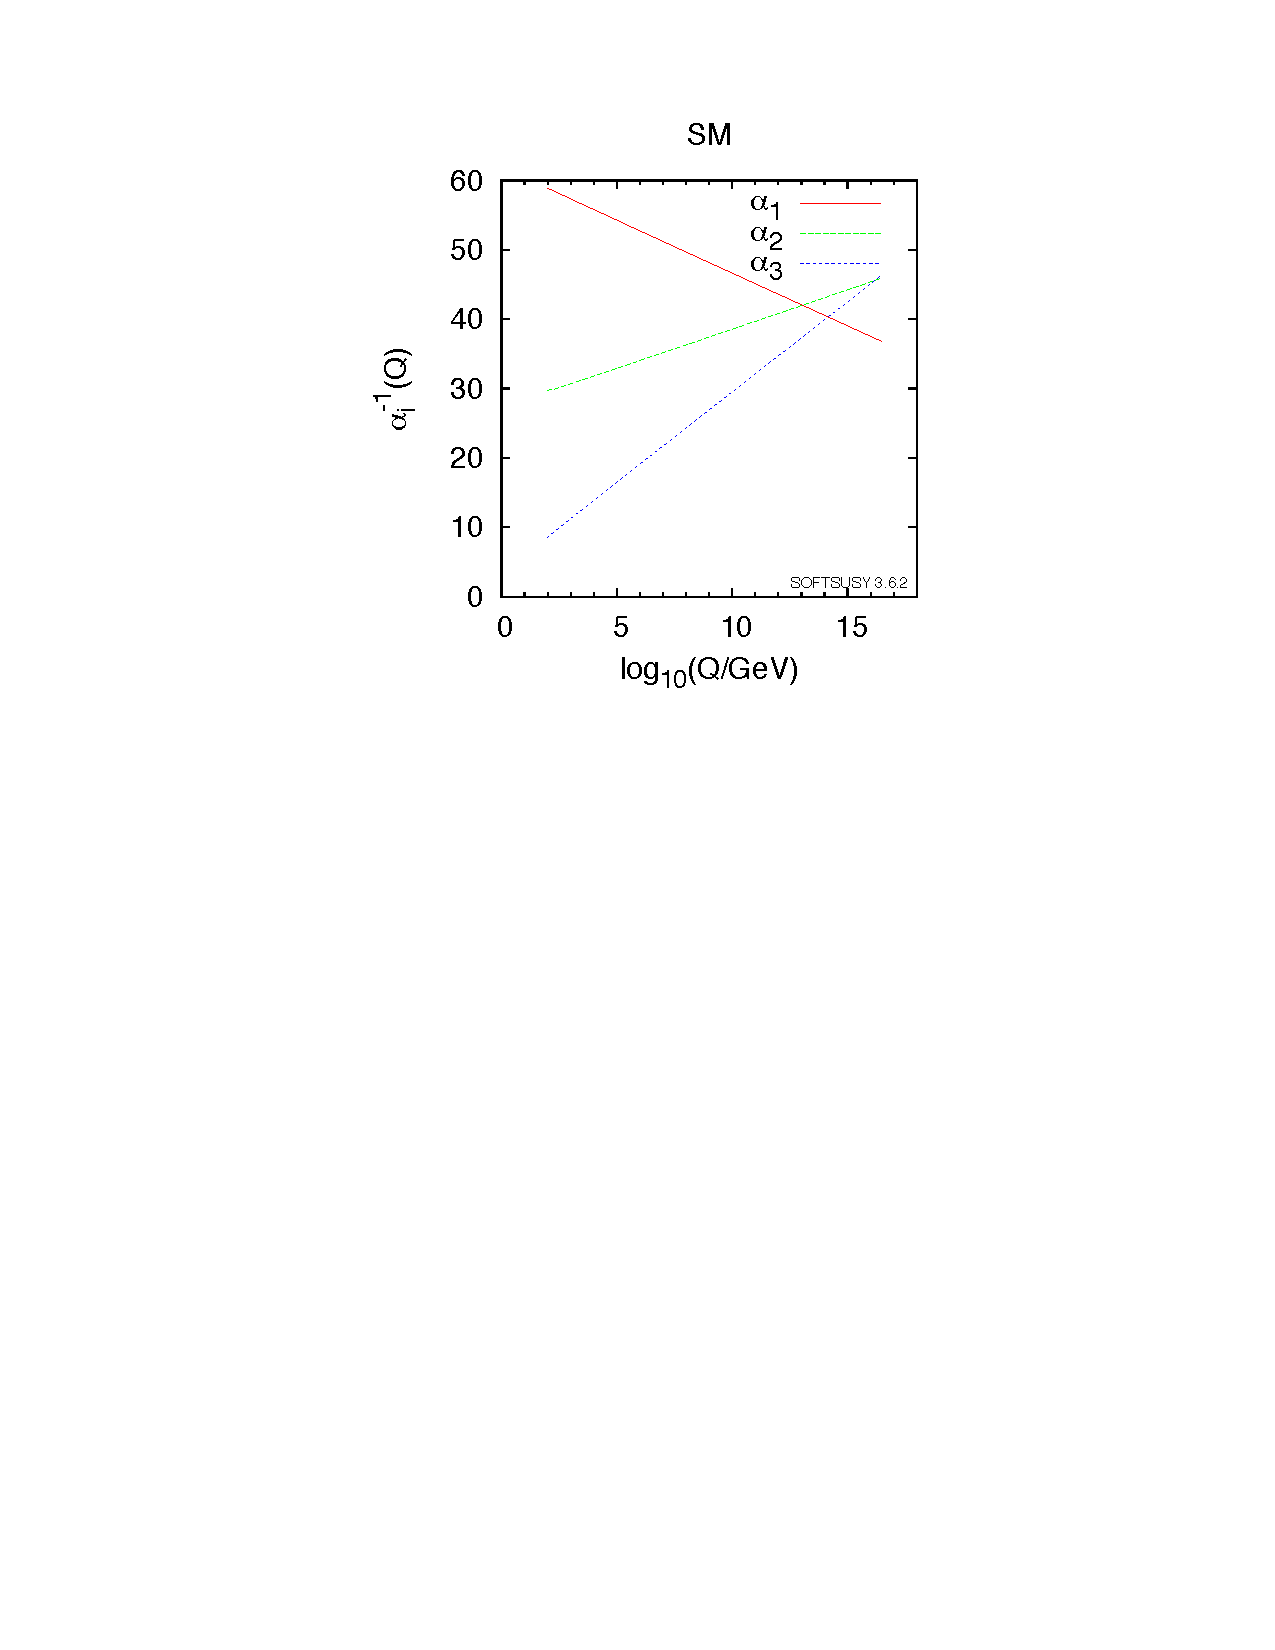
\includegraphics[width=0.49\textwidth]{figures/theory/gut_0.pdf}}
\subfigure[]{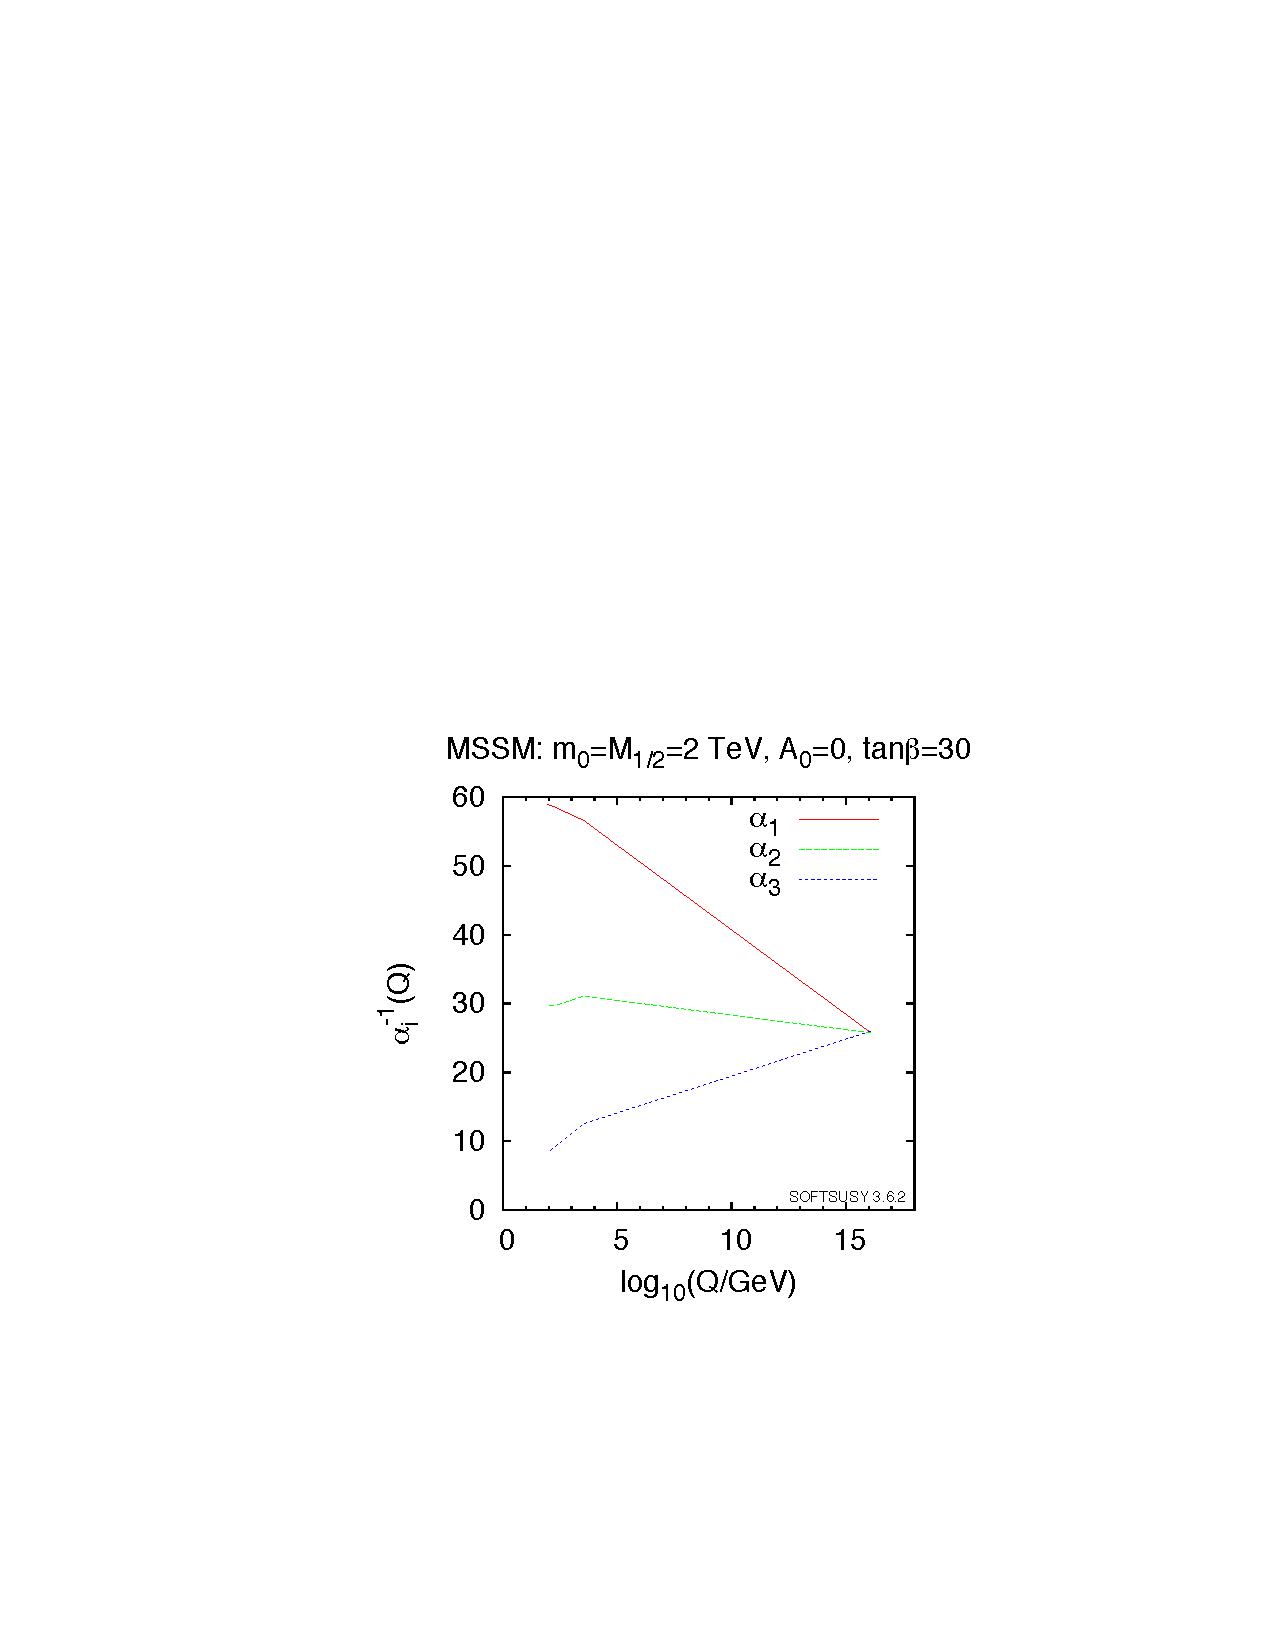
\includegraphics[width=0.49\textwidth]{figures/theory/gut_1.pdf}}
\caption{Running couplings in SM and MSSM, figure from Ref. \cite{Patrignani:2016xqp}.}
\label{fig:susy:gut}
\end{figure}

\subsubsection{Minimal Supersymmetric Standard Model}

SUSY is a framework that allows to generate an infinite number of models. The Minimal Supersymmetric Standard Model (MSSM) is the one that allows to include and extend the SM with the smallest amount of extra parameters, and is based on the \textit{superpotential}:

\begin{equation}
\begin{aligned}
W_{MSSM} & = y_u \tilde{u} \tilde{Q} H_u - y_d \tilde{d}\tilde{Q} H_d - y_e \tilde{e} \tilde{L}H_d + \mu H_u H_d \\  
& = \sum_{F, G, T} y_u^{FG} \tilde{u}_F \tilde{Q}_G^T H_u^T -
 = \sum_{F, G, T} y_u^{FG} \tilde{u}_F \tilde{Q}_G^T H_u^T - 
   \sum_{F, G, T} y_d^{FG} \tilde{d}_F \tilde{Q}_G^T H_d^T   \\ 
   & -
   \sum_{F, G, T} y_e^{FG} \tilde{e}_F\tilde{L}_G^T H_d^T  +
   \sum_{T} \mu H_u^T H_d^T 
\end{aligned}
\label{eq:WMMS}
\end{equation}

The superpotential appears in the MSSM Lagrangian through first and second order derivatives as discussed e.g. in Ref. \cite{Martin:1997ns}.

\renewcommand{\arraystretch}{1.4}
\begin{table}[h]
\begin{center}
\begin{tabular}{c c c c c}
\hline
\multicolumn{2}{c}{Names} 
& spin 0 & spin 1/2 & $SU(3)_C ,\, SU(2)_L ,\, U(1)_Y$
\\  \hline\hline
squarks, quarks & $Q$ & $({\tilde{u}}_L\>\>\>{\tilde{d}}_L )$&
 $(u_L\>\>\>d_L)$ & $(\>{\bf 3},\>{\bf 2}\>,\>{1d\over 6})$
\\
($\times 3$ families) & $\bar{u}$
&${\tilde{u}}^*_R$ & $u^\dagger_R$ & 
$(\>{\bf \overline 3},\> {\bf 1},\> -{2\over 3})$
\\ & $\bar{d}$ &${\tilde{d}}^*_R$ & $d^\dagger_R$ & 
$(\>{\bf \overline 3},\> {\bf 1},\> {1\over 3})$
\\  \hline
sleptons, leptons & $L$ &$({\tilde{\nu}}\>\>{\tilde{e}}_L )$&
 $(\nu\>\>\>e_L)$ & $(\>{\bf 1},\>{\bf 2}\>,\>-{1\over 2})$
\\
($\times 3$ families) & $\bar{e}$
&${\tilde{e}}^*_R$ & $e^\dagger_R$ & $(\>{\bf 1},\> {\bf 1},\>1)$
\\  \hline
Higgs, higgsinos &$H_u$ &$(H_u^+\>\>\>H_u^0 )$&
$(\tilde{H}_u^+ \>\>\> \tilde{H}_u^0)$& 
$(\>{\bf 1},\>{\bf 2}\>,\>+{1\over 2})$
\\ &$H_d$ & $(H_d^0 \>\>\> H_d^-)$ & $(\tilde{H}_d^0 \>\>\> \tilde{H}_d^-)$& 
$(\>{\bf 1},\>{\bf 2}\>,\>-{1\over 2})$
\\  \hline
\end{tabular}
\caption{Chiral supermultiplets in the Minimal Supersymmetric Standard Model.
The spin-$0$ fields are complex scalars, and the spin-$1/2$ fields are 
left-handed two-component Weyl fermions. Table from Ref. \cite{Martin:1997ns}. \label{tab:chiral}}
\vspace{-0.6cm}
\end{center}
\end{table}



\renewcommand{\arraystretch}{1.55}
\begin{table}[h]
\begin{center}
\begin{tabular}{c c c c}
\hline
Names & spin 1/2 & spin 1 & $SU(3)_C, \> SU(2)_L,\> U(1)_Y$\\
\hline\hline
gluino, gluon &$ \tilde{g}$& $g$ & $(\>{\bf 8},\>{\bf 1}\>,\> 0)$
\\
\hline
winos, W bosons & $ \tilde {W}^\pm\>\>\> \tilde {W}^0 $&
 $W^\pm\>\>\> W^0$ & $(\>{\bf 1},\>{\bf 3}\>,\> 0)$
\\
\hline
bino, B boson &$\tilde{B}^0$&
 $B^0$ & $(\>{\bf 1},\>{\bf 1}\>,\> 0)$
\\
\hline
\end{tabular}
\caption{Gauge supermultiplets in
the Minimal Supersymmetric Standard Model. Table from Ref. \cite{Martin:1997ns}. \label{tab:gauge}}
\vspace{-0.45cm}
\end{center}
\end{table}

The chiral supermultiplets of the MSSM are described in Table \ref{tab:chiral}, and the gauge supermultiples in Table \ref{tab:gauge}. Note that the states defined in these tables are the interaction eigenstates, but not necessary mass eigenstates as mixing is possible. In particular, the higgsinos mix with the gauginos, as well as the sfermions associated with the left and right component of the same SM fermion. The gluinos instead do not undergo any mixing, as there are no other superpartners with the proper quantum numbers.


\subsubsection{SUSY Higgs Sector}
\label{sec:susy:higgs}

To maintain an holomorphic superpotential, SUSY requires at least two SU(2) doublets: one to give mass to up-type quarks ($H_u$) and one to give mass to the the down-type quarks ($H_d$). The two doublets provide 8 degrees of freedom. Three of them are the ones needed to give masses to the gauge bosons, while the other 5 become observable particles:
\begin{itemize}
\item Two CP-even neutral Higgs bosons: $h^0$ (the lighter) and $H^0$.
\item $A^0$, a CP-odd Higgs boson.
\item Two charged Higgs bosons, $H^+$ and $H^-$.
\end{itemize}


\subsubsection{Particle Content of the MSSM}

\subsubsection{R-parity}

\subsubsection{SUSY Breaking Terms}


% Supersymmetry (SUSY) is a BSM framework that allows to generate an infinite amount of BSM models, each with different signatures.
